% ****** Start of file RamanCoolingV1.tex ******
%
%
% See the REVTeX 4 README file
% It also requires running BibTeX. The commands are as follows:
%
%

\documentclass[%
 reprint,
%superscriptaddress,
%groupedaddress,
%unsortedaddress,
%runinaddress,
%frontmatterverbose, 
%preprint,
%showpacs,preprintnumbers,
%nofootinbib,
%nobibnotes,
%bibnotes,
 amsmath,amssymb,
 aps,
prl,
%pra,
%prb,
%rmp,
%prstab,
%prstper,
%floatfix,
]{revtex4-1}

\usepackage{graphicx}% Include figure files
\usepackage{dcolumn}% Align table columns on decimal point
\usepackage{bm}% bold math
%\usepackage{hyperref}% add hypertext capabilities
%\usepackage[mathlines]{lineno}% Enable numbering of text and display math
%\linenumbers\relax % Commence numbering lines

%\usepackage[showframe,%Uncomment any one of the following lines to test 
%%scale=0.7, marginratio={1:1, 2:3}, ignoreall,% default settings
%%text={7in,10in},centering,
%%margin=1.5in,
%%total={6.5in,8.75in}, top=1.2in, left=0.9in, includefoot,
%%height=10in,a5paper,hmargin={3cm,0.8in},
%]{geometry}

\begin{document}

%\preprint{APS/123-QED}

\title{A Plugged Trap for Crossed Field Spin-Flip Loss}%


\author{David Reens}%
\author{Hao Wu}
\author{Tim Langen}%
\author{Jun Ye}
\affiliation{%
 Physics Department, University of Colorado at Boulder\\
}%

\date{\today}% It is always \today, today,


%%%%%%%%%%%%%%%%%%%%%
%ABSTRACT
%%%%%%%%%%%%%%%%%%%%%
\begin{abstract}
A new electromagnetic trap geometry allows tunable plugging of non-adiabatic spin flip loss in crossed electric and magnetic fields. This loss afflicts a wide set of candidate molecules and operates at much higher temperatures compared with the more familiar atomic spin-flip loss near the zero of a magnetic trap, and thus it's removal represents an important step toward quantum degenerate molecules. Using only an external magnetic bias coil, the loss rate is tuned from over $100 \text{ s}^{-1} $ to below the vacuum limited lifetime in a $100 \text{ mK}$ sample of OH molecules.
\end{abstract}


\maketitle


%%%%%%%%%%%%%%%%%%%%%%%%%%%%%%%%%
%
%     III   NNN   TTT   RRR   OOO   DDD   UUU   CCC   TTT   III   OOO   NNN
%     III   NNN   TTT   RRR   OOO   DDD   UUU   CCC   TTT   III   OOO   NNN
%     III   NNN   TTT   RRR   OOO   DDD   UUU   CCC   TTT   III   OOO   NNN
%
%%%%%%%%%%%%%%%%%%%%%%%%%%%%%%%%%
\section{Introduction}
Quantum degenerate atomic ensembles continue to support an impressive array of frontier research in fundamental quantum statistics, condensed matter simulations, and precision measurement. The greatly anticipated extension to molecular ensembles continues to move forward, with progress on all fronts- direct, indirect, electromagnetic, optical, or combinations thereof. The benefits of molecules are closely paired with new challenges. The electric dipole moment, perhaps the most anticipated molecule characteristic, requires the presence of nearby opposite parity states which can complicate optical pumping schemes, serve as inelastic collision channels, or even dramatically enhance spin-flip trap losses. These molecule specific challenges are being systematically addressed with novel optical pumping and magneto-optical trapping schemes, non-optical cooling techniques, field-suppressed inelastic collisions, and with regard to enhanced spin-flip losses, with the trap geometry strategy here reported. 

The knowledge of spin flips or Majorana hops as an eventual trap lifetime limit predates the very first magnetic trapping of neutrals\cite{Migdall1985}. Spin flips were directly observed and overcome in the TOP trap\cite{Petrich1995}, and shortly later with a plugged dipole trap\cite{Davis1995}, famously enabling the first quantum degenerate atomic ensembles. The molecular spin-flips can occur at much higher temperatures compared with their atomic counterpart, and thus they need to be addressed much earlier than might have been expected. The magnitude of the loss varies with molecular species, and is particularly strong for the case of the OH molecule used here, but is nonetheless remarkably general.

In section two, we will thoroughly explain this crossed field spin flip loss mechanism and it's applicability to other molecules, before describing our new electromagnetic trap geometry in section three. In section four we provide our experimental evidence and then conclude.


%%%%%%%%%%%%%%%%%%%
%  EXPLAIN THE LOSS MECHANISM
%%%%%%%%%%%%%%%%%%%
\section{Loss Mechanism  \label{sec:lm} }
Successful trapping is predicated on the adiabatic criterion that the internal state of the trapped species is decoupled from the trapping geometry and maintains its quantization direction despite slow changes in the magnitude and direction of the field providing said quantization. Conversely, this fails whenever the variation in the external field is too fast, in which case the adiabatic criterion is not satisfied and the state may flip to an un-trapped one. Near the zero of a magnetic quadrupole trap, the direction of the field can change rapidly, leading to this breakdown, which we call spin-flip loss.

An equivalent description of spin-flip loss focuses on the proximity of other states to the primary trapped state. When other states are nearby in energy to the trapped one, it becomes possible to hop to them, and since the external field breaks the degeneracy between these states, when it is small hops are possible, again near the zero of a magnetic quadrupole trap. The exact formulation for the simplest system first performed by Majorana shows that both descriptions contribute, and hopping probability is proportional to the exponent of energy gap between nearby states divided by the rate of change of the state energy:

\begin{equation}
P_{\text{LZ}}=e^{-\Delta^2/E'}
\end{equation}

Although this only applies exactly in the case of two states and a linear tuning of the external field from minus to plus infinity, in practice it can be applied whenever only two states are nearby and they approach linearly with time close to a crossing. 

To understand the enhanced trap loss for dipolar molecules, we first consider a molecule in homogeneous fields. For Hund's case (a) molecules, as described in \cite{Lara2008}, the Stark and Zeeman perturbations are not mutually diagonal, and thus the effects combine differently depending on the angle between the fields. With parallel fields the effects are purely additive, but with perpendicular fields they are less so. In fact, the presence of one field can be thought of as ``blocking" the effect of the second field when it is much smaller than the first. In Fig.~\ref{fig:starkzeemanlines}, the Zeeman effect in the presence of an orthogonal electric field is compared to that with a parallel field of the same magnitude and without any electric field. It is seen that the electric field blocks the zeeman effect from linear to cubic for ground state $^2\Pi_{3/2}$ weak field seeking OH:

\begin{equation}
H_Z\propto \frac{B^3}{E^4}f(\Delta,E)\Delta
\end{equation}

Here $B$, $E$, and $\Delta$ are Zeeman, Stark, and lambda doublet energies with all coefficients subsumed. $f$ is a function of lambda doublet and stark energy with units of energy that approaches $\Delta$ for $E << \Delta$ but $E$ for large $E$. Thus in any magnetic trap where electric field exists near a magnetic field zero, states will be close to one another in a larger region than otherwise because the zeeman effect is blocked from linear to cubic and extra magnetic field is required to break the degeneracy. More precisely, let $\kappa$ be the threshold for gaps between states below which spin-flips are possible at say the 1\% level. $\kappa$ depends on the velocity of trapped species, but suppose we have a specific temperature of interest, and therefore a mean velocity. Without electric field, the effective cross sectional area for a hopping region is $\pi \kappa^2$, since loss can occur where $B<\kappa$. With electric field, we have

\begin{equation}
B < \sqrt[3]{\frac{\kappa E^4}{f(\Delta,E)\Delta}}
\end{equation}

With $E<<\kappa$ there is no enhancement. (Nor is there any reduction, the Zeeman effect returns to linear by the time $B$ reaches $\kappa$. For $E>\sqrt[4]{\kappa^2\Delta f(\Delta,E)}~\sqrt{\kappa\Delta}$, there is an enhancement. We can assume $E<\Delta$ since $\kappa<<\Delta$ at temperatures of interest. In terms of loss area, the enhancement factor is given by:

\begin{equation}
\nu = \left(\frac{E^4}{\kappa^2\Delta^2}\right)^\frac{2}{3}\label{eq:blimit}
\end{equation} 

It is interesting to note that in ref.~\cite{Lara2008}, it was specifically undertaken to investigate the spin-flip loss for OH molecules in a magnetic quadrupole trap with superposed electric field, and no enhancement was found. This turns out to be a consequence of a reasonable yet false assumption that a 4-state approximate Hamiltonian with two spin states and two parities would contain the behavior relevant for spin-flip loss in mixed fields. This approximate Hamiltonian exhibits only constant order blocking- i.e. the Zeeman effect remains linear though with adjusted slope. This is intuitively reasonable, because with two spin states, the Zeeman effect has to break the Stark effect's coupling of opposite spin states, a 1st order task, but a 3rd order when there are 4 spin states and the states coupled by the Stark effect are three magnetic quanta apart. More recent work in our lab correctly recognized the importance of the effect and accounted for it, although this was done numerically with no algebraic interpretation.

This effect will influence any case (a) molecule with more than two magnetic states such as NO ($X^2\Pi_{3/2}$), and it will also influence case (b) molecules in accordance with the strength of their non-zero spin-rotation coupling often denoted $\gamma$. (I'd like to check how much this enhances loss for YO and SrF, but I haven't done it yet). It also might crop up with superposed optical and magnetic fields, though I haven't tried to check.

%%%%%%%%%%%%%%%%%%%%%%%%%%
%  PIN TRAP GEOMETRY
%%%%%%%%%%%%%%%%%%%%%%%%%%
\section{Pin Trap Geometry \label{sec:ptg} }
One obvious way to avoid the loss enhancement is to simply never use electric field in a magnetic trap. This prevents loss from being enhanced compared with atoms, but doesn't remove it entirely. Another possibility is to trap with electric fields, where no spin-flip loss is possible thanks to the large lambda-doublet splitting. However this splitting also results in a significant reduction in trap gradient close to the trap center, very undesirable for further cooling by evaporation, which needs as much phase space density as possible.

Another option would be to apply electric fields nowhere orthogonal to magnetic, for example overlapped quadrupole fields. In this case the loss is neither enhanced nor entirely removed, but perfect alignment is required. If the zeros do not overlap, there is a loss region whose size is set by the misalignment. 

Seeking to remove the loss entirely but without any trap gradient sacrifice, we developed a solution that requires devoting both electric and magnetic fields to trapping, but is in all other respects a best-case scenario. Instead of avoiding orthogonal fields entirely, the geometry simply ensures that the magnetic field is not too close to zero when they are orthogonal. The key idea is to use a 2D instead of a 3D magnetic quadrupole, apply a homogeneous bias magnetic field in the untrapped direction to prevent the magnetic field from having any zeros, and trap in the third direction with electric fields. The fields can be approximated as follows:

\begin{eqnarray}
\vec{B} &=&  B^\prime y\hat{x}+ B^\prime x\hat{y} + B_{coil} \hat{z}\\
\vec{E} &=&  E^\prime y\hat{y}-  E^\prime z\hat{z}
\end{eqnarray}

In other words 2D quadrupole traps in the xy plane for B and in the yz plane for E. Now E is perpendicular to B when:
\begin{eqnarray}
\vec{B}\cdot \vec{E} &= 0\\
B^\prime x E^\prime y - B_{coil}  E^\prime z &= 0\\
B_{coil}z &= xyB^\prime
\end{eqnarray}

So we see that E and B are perpendicular on a hyperbolic sheet which deviates more significantly from the z axis with increasing $B_{coil}$, and reduces to the pair of planes $x=0$ and $y=0$ in the limit that $B_{coil} = 0$. On this hyperbolic sheet, B must be larger than the threshold set by Eq.~\ref{eq:blimit}. In fact, the volume everywhere in which the limit is satisfied can be directly solved. 

\begin{equation}
|B|^3 = \left(B'^2(x^2+y^2)+B_{\text{coil}}^2\right)^3 < \begin{cases} \kappa E'^4(y^2+z^2)^2/\Delta^2,  E'\sqrt(y^2+z^2)<\Delta\\ E'^3(y^2+z^2)^{3/2} /\Delta, E'\sqrt(y^2+z^2)>\Delta\end{cases}
\end{equation}

In our experiment, $B' \approx 5 \text{T/cm} \times 1.4\mu_\text{B}$, and $E' ~ 120 \text{kV/cm}^2 \times 1.67 d_E$, so $B'/E' ~ 1$. 

When $B\cdot E = 0$, the B field must be larger than the limit where $\mu_eE >> \mu_b B$, i.e. close to the z-axis since that is where $B$ is small, and further from $z=0$ since that is where $E$ is large. You can see the loss regions plotted as a function of $B_{coil}$, with $B_{pin}$ set to zero in Fig.~\ref{fig:LSurfs}.

Notably, $B_{coil}$ tunes the proximity of the loss regions to the trap center, and is thus potentially useful as a knife for spectroscopy or evaporation.

\begin{figure}[b]
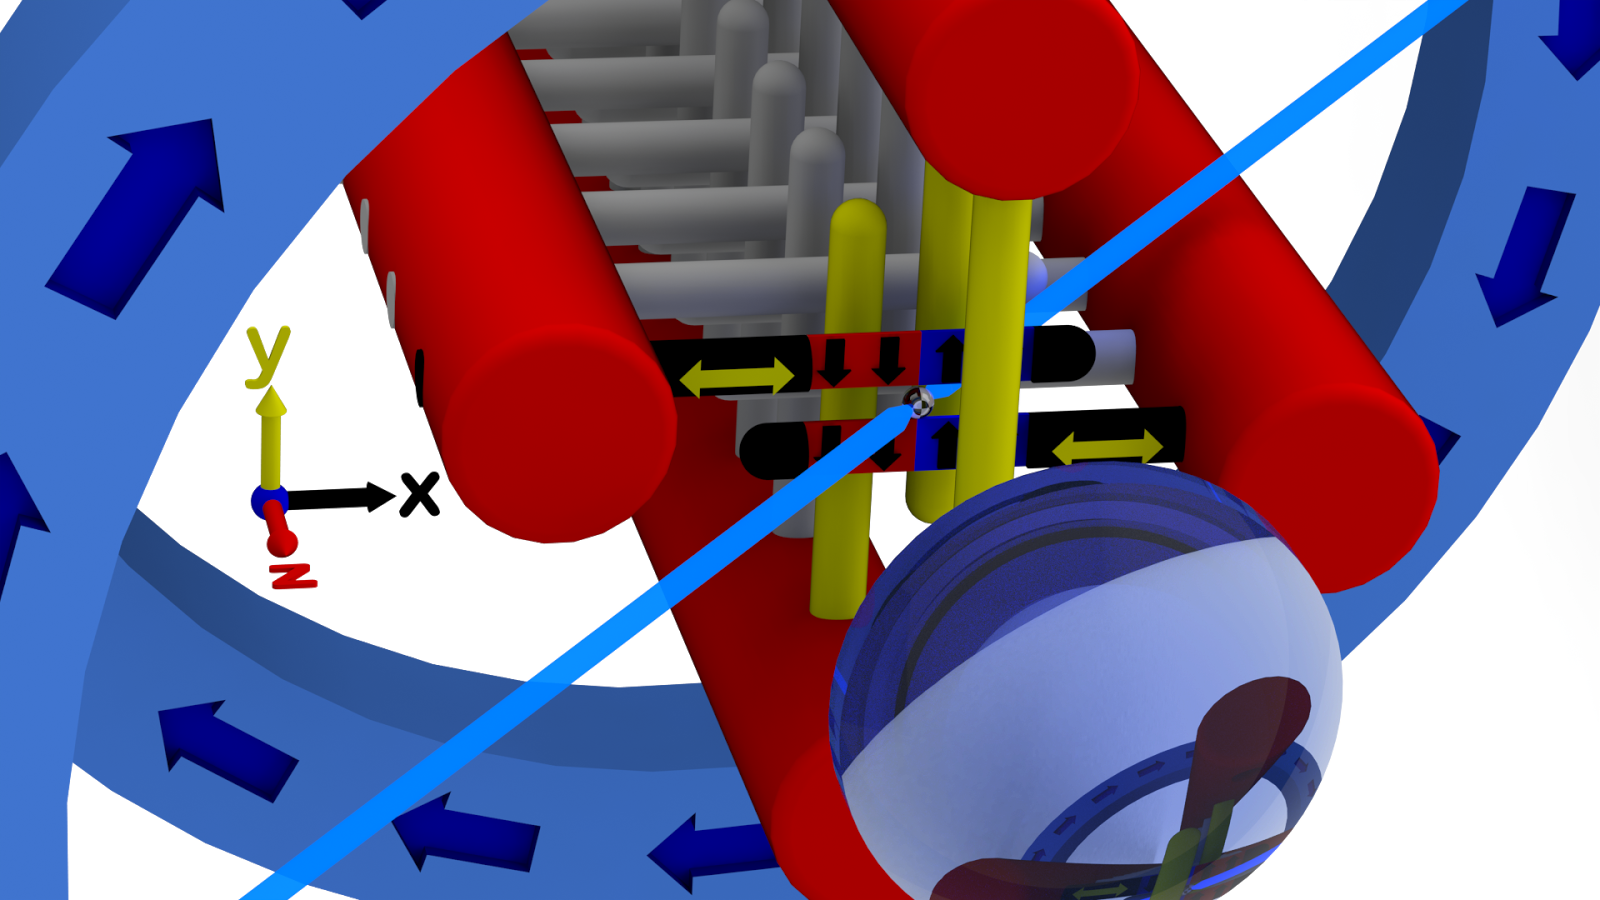
\includegraphics[width=70mm]{blue-red-yellow-v2_CAD.png}%
\caption{
OH molecules are created using a supersonic expansion source and decelerated from an initial velocity of 460m/s to a final velocity of 40ms/s using a Stark decelerator (red). The decelerator contains 142 electrode pairs (gray). Trapping is achieved by combining a radial magnetic quadrupole field, created by the magnetized second to last electrode pair of the decelerator, with a longitudinal electric quadrupole field created by the third to last and last electrode pairs, respectively (yellow, one electrode is omitted for clarity). The magnetized electrodes can be translated in situ along the x-axis to align their domains and optimize the quadrupole. As there is no trapping magnetic field in the z-direction in this configuration, macroscopic external bias coils can be used to lift the gap between the top two states of the OH ground-state manifold and thus tune the molecular loss. Detection is realized using laser induced fluorescence along the x+y-z direction (blue), which is collected using a lens system and PMT in the z-direction.
\label{fig:CAD}}
\end{figure}


\begin{figure}[b]
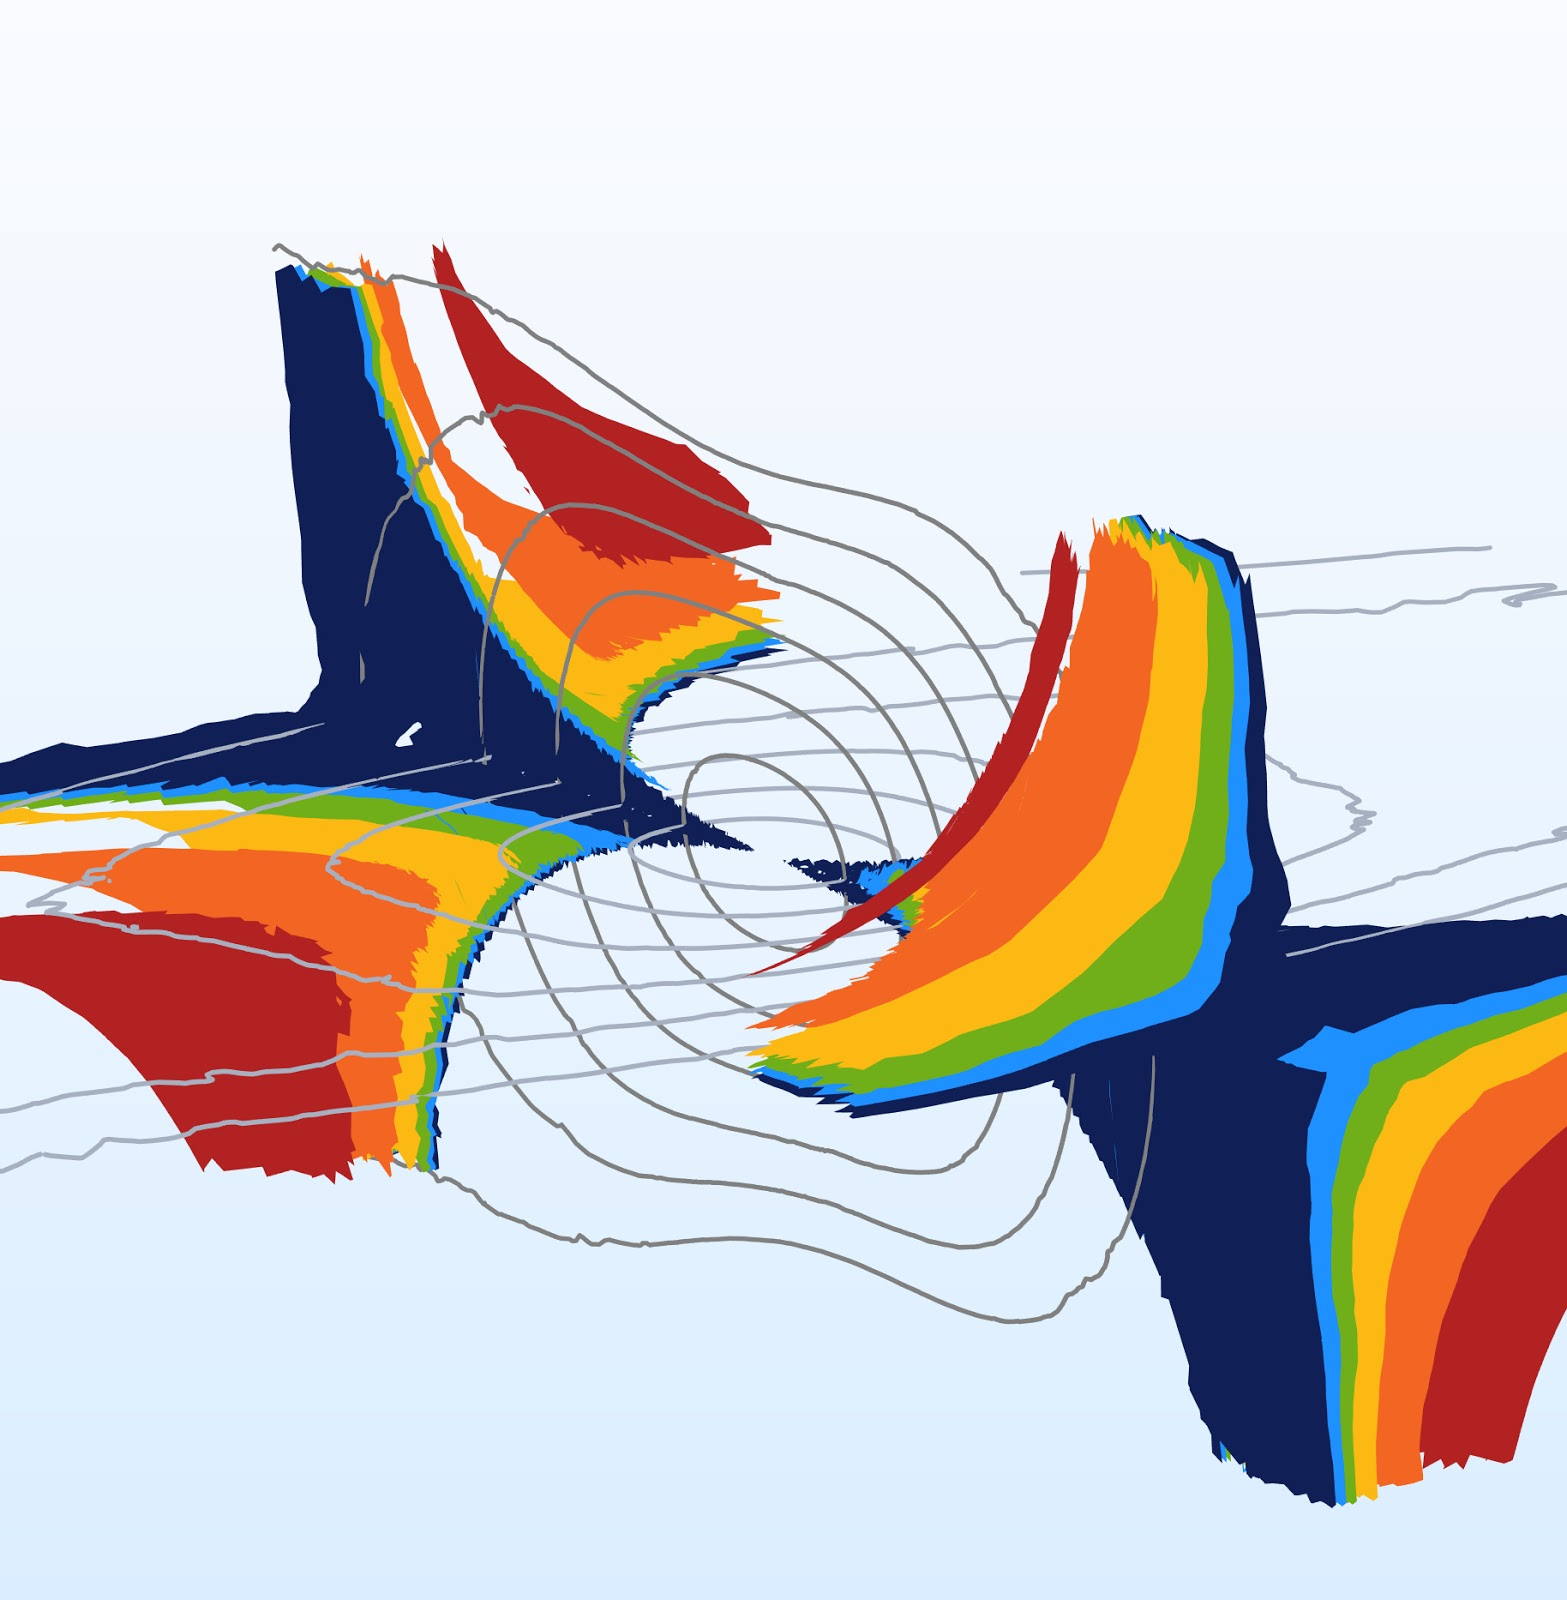
\includegraphics[width=70mm]{Loss_Surface_Chunks_0-320_0.jpeg}%
\caption{
Contours every 100mK, colors 0,20,40,80,160,320 G bias field and pin offset at zero. Molecules can spin-flip and be lost, whenever they cross these areas.
\label{fig:LSurfs}}
\end{figure}

%%%%%%%%%%%%%%%%%%%
%  LOSS TRAJECTORY DATA
%%%%%%%%%%%%%%%%%%%
\section{Loss Trajectories}
We can measure OH population in the trap as a function of time and as a function of bias field used for removing the loss. This demonstrates how truly wonderful and amazing we are.


%includes uncited bib entries
\nocite{*}


\bibliography{MolecularMajoranaLoss.bib}% Produces the bibliography via BibTeX.

\end{document}
%
% ****** End of file MolecularMajoranaLoss.tex ******
